        %%******************************************%%
        %%                                          %%
        %%        Modello di tesi di laurea         %%
        %%            di Andrea Giraldin            %%
        %%                                          %%
        %%             2 novembre 2012              %%
        %%                                          %%
        %%******************************************%%

\begin{document}
    \frontmatter
    \begin{titlepage}
    \begin{center}
        \begin{LARGE}
            \textbf{\myUni}\\
        \end{LARGE}

        \vspace{10pt}

        \begin{Large}
            \textsc{\myDepartment}\\
        \end{Large}

        \vspace{10pt}

        \begin{large}
            \textsc{\myFaculty}\\
        \end{large}

        \vspace{30pt}
        \begin{figure}[htbp]
            \centering
            
\includegraphics[height=6cm]{unipd-logo}
        \end{figure}
        \vspace{30pt}

        \begin{LARGE}
            \textbf{\myTitle}\\
        \end{LARGE}

        \vspace{10pt}

        \begin{large}
            \textsl{\myDegree}\\
        \end{large}

        \vspace{40pt}

        \begin{large}
            \begin{flushleft}
                \textit{Relatore}\\
                \vspace{5pt}
                \profTitle\ \myProf \\
                \vspace{5pt}
                \textit{Correlatore}\\
                \tutorTitle\ \myTutor
            \end{flushleft}

            % You can tweak the spacing to have professor and student names on the same line
            % useful if the page is broken by a long thesis title and you need more space
            \vspace{-70pt}

            \begin{flushright}
                \textit{Laureando}\\
                \vspace{5pt}
                \myName \\
                \vspace{5pt}
                \textit{Matricola} \myID
            \end{flushright}
        \end{large}

        \vspace{40pt}

        \line(1, 0){338} \\
        \begin{normalsize}
            \textsc{Anno Accademico \myAA}
        \end{normalsize}
    \end{center}
\end{titlepage}

    \clearpage
\phantomsection
\thispagestyle{empty}

\hfill
\vfill

\noindent\myName: \textit{\myTitle,}
\myDegree,
\textcopyright\ \myTime.

    \cleardoublepage
\phantomsection
\thispagestyle{empty}
\pdfbookmark{Dedica}{Dedica}

\vspace*{3cm}

\begin{center}
    Lorem ipsum dolor sit amet, consectetuer adipiscing elit. \\ \medskip
    --- Oscar Wilde
\end{center}

\medskip

\begin{center}
    Dedicato a ...
\end{center}

    \cleardoublepage
\phantomsection
\pdfbookmark{Sommario}{Sommario}
\begingroup
\let\clearpage\relax
\let\cleardoublepage\relax
\let\cleardoublepage\relax

\chapter*{Sommario}

Il presente documento descrive il lavoro svolto durante il periodo di stage, della durata complessiva di trecentoventi ore, dal laureando Giovanni Menon presso l'Università degli studi di Padova.
Il tirocinio è stato condotto sotto la guida del Prof. Alessandro Galeazzi e con la collaborazione del Dott. Enrico Bassetti.
Il Prof. Davide Bresolin ha ricoperto il ruolo di tutor accademico e referente interno al Consiglio del Corso di Studio.
\\\\
Questa tesi riguarda l'analisi del protocollo \emph{Quick UDP Internet Connections (QUIC)} nel contesto delle reti moderne, 
con particolare attenzione alle problematiche legate alla tariffazione del traffico dati. Lo studio ha esplorato alcune possibili strategie che potrebbero
essere sfruttate per manipolare artificialmente il traffico mobile. 
I risultati ottenuti hanno evidenziato come queste strategie possano indurre un incremento del traffico dati per l'utente vittima, 
aumentando di conseguenza i suoi consumi dati e i suoi relativi costi. 
\\\\
Il tirocinio si è suddiviso in due parti.
La prima dedicata ad un'analisi approfondita del protocollo \emph{QUIC}, esaminando non solo lo stato dell'arte attuale e le tecnologie associate, ma anche la sua logica intrinseca e il suo funzionamento.
La seconda parte, invece, si è concentrata sulla progettazione e realizzazione degli esperimenti volti a testare le strategie identificate, terminando nella raccolta e nell'analisi dei risultati ottenuti.
%\vfill

%\selectlanguage{english}
%\pdfbookmark{Abstract}{Abstract}
%\chapter*{Abstract}

%\selectlanguage{italian}

\endgroup

\vfill

    \cleardoublepage
\phantomsection
\pdfbookmark{Ringraziamenti}{ringraziamenti}

\bigskip

\begingroup
\let\clearpage\relax
\let\cleardoublepage\relax
\let\cleardoublepage\relax

\chapter*{Ringraziamenti}

\textit{Giunto alla fine di questo percorso accademico, desidero esprimere la mia profonda riconoscenza verso tutti coloro che mi hanno sostenuto e che ho avuto la fortuna di incontrare.}
\\\\
\noindent \textit{In primis, desidero esprimere la mia più profonda gratitudine al Prof. \myProf, relatore di questa tesi, per il suo prezioso supporto durante l'intero processo di stesura. Un sentito ringraziamento va anche al Dott. \myTutor, la cui supervisione durante il tirocinio e i cui consigli si sono rivelati una guida fondamentale per la realizzazione di questo lavoro.}
\\\\
\noindent \textit{Un ringraziamento speciale va ai miei genitori, Maria Teresa e Doriano, e a mio fratello Francesco, per avermi sostenuto, incoraggiato e sopportato durante questo percorso. 
Un grazie particolare ai miei genitori, i cui sacrifici mi hanno dato l'opportunità di intraprendere e completare questo percorso.}
\\\\
\noindent \textit{Un caloroso ringraziamento va alle mie nonne, Angela e Luciana, che con il loro affetto mi sono state vicine durante questi tre anni di studi.}
\\\\
\noindent \textit{Un grazie speciale va ai miei più cari amici Jacopo, Davide e Marco, presenze costanti in ogni momento di questo percorso. La vostra vicinanza, il vostro sostegno e la vostra capacità di spronarmi a dare il meglio di me sono stati fondamentali.}
\\\\
\noindent \textit{Un grazie a tutti coloro che ho conosciuto lungo questo percorso. In particolare ringrazio i ragazzi di CodingCowboys e i miei amici del Concilio per essere stati una compagnia costante in questi anni di studio.}
\bigskip

\noindent\textit{\myLocation, \myTime}
\hfill \myName 

\endgroup

    \cleardoublepage
\pdfbookmark{\contentsname}{tableofcontents}
\setcounter{tocdepth}{2}
\tableofcontents
%\markboth{\contentsname}{\contentsname}
\clearpage

\begingroup
    \let\clearpage\relax
    \let\cleardoublepage\relax
    \let\cleardoublepage\relax

    % Figures list
    \phantomsection
    \pdfbookmark{\listfigurename}{lof}
    \listoffigures

    \vspace*{8ex}

    % Tables list
    \phantomsection
    \pdfbookmark{\listtablename}{lot}
    \listoftables

    \vspace*{8ex}
\endgroup

\cleardoublepage

    \cleardoublepage

    \mainmatter
    \chapter{Introduzione}
\label{cap:introduzione}

(Bozza)\\\\
\emph{Abstract}- L'adozione di nuovi protocolli come \emph{Quick UDP Internet Connections (QUIC) } nelle reti moderne ha introdotto nuove sfide nella gestione e tariffazione del traffico.
Questo studio si concentra sull'analisi di questo protocollo con particolare attenzione alle problematiche relative alla tariffazione dei consumi e alle possibili tecniche per aumentare il traffico.
Si sono analizzate tre diverse strategie per la manipolazione del traffico: (1) un server malevolo che agisce come se non ricevesse alcun ACK e con un PTO costante a zero, (2) l'inserimento silenzioso di 
pacchetti aggiuntivi da parte del server durante una comunicazione, e (3) un attacco esterno che manipola il traffico mascherando selettivamente alcuni pacchetti.
Attraverso lo studio di queste strategie sono stati esaminati i risultati ottenuti. Lo studio ha evidenziato come queste strategie possano portare ad un aumento del traffico e 
dei consumi.


\section{Motivazione}
L'avvento di Internet e la continua evoluzione delle tecnologie di comunicazione ha trasformato radicalmente il modo di interagire e accedere alle informazioni.
Tuttavia, tale progresso porta con sè nuove sfide nella gestione e tariffazione del traffico.
I piani tariffari attuali, basati su soglie o sui consumi effettivi, si affidano al calcolo del consumo dati effettuato dagli operatori di rete.
Questo approccio, tuttavia, introduce una serie di nuove problematiche. Un esempio significativo è rappresentato 
dalla possibilità che un malintenzionato potrebbe sfruttare le caratteristiche intrinseche di un protocollo di rete o del sistema di comunicazione 
per manipolare artificialmente il consumo dati degli utenti senza che questi ne siano consapevoli.
Ciò comporta un aumento del costo o l'esaurimento prematuro delle risorse dati disponibili.
Risulta quindi necessario analizzare le possibili strategie utilizzate e valutare gli impatti che queste potrebbero avere sugli utenti.

\section{Organizzazione del testo}
\indent Di seguito, viene presentata la struttura del documento :
\begin{description}
    \item[{\hyperref[cap:RelatedWorks]{Il secondo capitolo}}] presenta quanto trovato di simile nella letteratura attuale;

    \item[{\hyperref[cap:descrizione]{Il terzo capitolo}}] approfondisce il background e illustra l'idea del progetto;
    
    \item[{\hyperref[cap:processi-metodologie]{Il quarto capitolo}}] descrive dettagliatamente l'ambiente di sviluppo e presenta i singoli esperimenti condotti;

    \item[{\hyperref[cap:risultati]{Il quinto capitolo}}] riassume e analizza i risultati ottenuti dagli esperimenti;
    
    \item[{\hyperref[cap:conclusioni]{Il sesto capitolo}}] presenta le conclusioni del lavoro e propone possibili sviluppi futuri.
\end{description}

    \chapter{Processi e Metodi}
\label{cap:processi-metodologie}

\textit{\indent Questo capitolo fronisce in dettaglio l'ambiente di ricerca adottato, le tecnologie impiegate e degli esperimenti condotti. 
Fornisce inoltre tutte le informazioni necessarie per replicare gli esperimenti.}

\section{Ambiente}
~\\
\indent Questa sezione offre una panoramica completa dell'ambiente di lavoro e delle tecnologie impiegate nello sviluppo degli esperimenti descritti successivamente. 
Segue una descrizione degli strumenti utilizzati durante lo svolgimento del progetto (riassunte con le relative versioni nella Figura \ref{table-tecnologie}).
\\\\
Come premessa, la totalità del progetto è stata svolta su \textbf{\emph{Ubuntu}}\footnote{\url{https://ubuntu.com/}}. 
Questa scelta di sistema operativo è dovuta al vasto supporto di strumenti per l'analisi e lo sviluppo.
\\\\
Per l'analisi del traffico di rete, è stato ampiamente utilizzato \textbf{\emph{Wireshark}}\footnote{\url{https://www.wireshark.org/}}, 
uno strumento molto diffuso nel panorama del traffico di rete e che ha permesso di esaminare nel dettaglio il comportamento dei protocolli oggetti dello studio.
\\\\
La sperimentazione ha coinvolto l'uso di diversi \emph{browser web}, in particolare \textbf{\emph{Google Chrome}}\footnote{\url{https://www.google.com/intl/it_it/chrome/}} e \textbf{\emph{Firefox}}\footnote{\url{https://www.mozilla.org/it/firefox/}}. 
Questi due applicativi sono stati impiegati per testare e confrontare l'implementazione dei protocolli in diverse situazioni.
\\\\
L'ambiente di test è stato realizzato tramite \textbf{Oracle VM VirtualBox}\footnote{\url{https://www.virtualbox.org/}}, un diffuso ambiente di virtualizzazione. 
Permettendo di creare e gestire macchine virtuali specifiche per la creazione di possibili scenari.
\\\\
Per la condivisione e mantenimento del codice si è usato \textbf{GitHub}\footnote{\url{https://github.com/}} e \textbf{Git}.
In particolare si è rivelato vantaggioso in quanto ha permesso di lavorare efficientemente con \emph{fork}\footnote{\gls{fork}} di librerie pubbliche, consentendo una gestione dinamica delle modifiche e degli aggiornamenti del codice.

\subsection{Tecnologie Specifiche per QUIC}
~\\
\indent Per lo studio si è utilizzato \textbf{Quic-go}\footnote{\url{https://github.com/quic-go/quic-go}}, un'implementazione sviluppata in \emph{Go}\footnote{\gls{Go}} del protocollo \emph{QUIC}.
\emph{Quic-go} è un progetto \emph{open source} su \emph{GitHub} che aderisce rigorosamente alle specifiche del protocollo \emph{QUIC} 
definite negli \emph{RFC}\footnote{\gls{RFC}} 9000, 9001 e 9002. 
\\\\
\emph{Quic-go} non è l'unica versione disponibile del protocollo \emph{QUIC}.
Come illustrato nella Figura \ref{table-implementazioni-quic}, esistono numerose altre implementazioni, sia \emph{open source} che proprietarie, ciascuna cerca di rispettare rigorosamente le specifiche definite negli \emph{RFC}. 
\\\\
La scelta di utilizzare questa specifica implementazione di \emph{QUIC} è motivata dal suo utilizzo all'interno di \textbf{Caddy}\footnote{\url{https://caddyserver.com/}}, un \emph{web server} moderno e performante. \emph{Caddy} integra \emph{Quic-go} per offrire il supporto nativo del protocollo \emph{QUIC} e \emph{HTTP/3}.
Inoltre, si è utilizzato \textbf{xCaddy}, un \emph{tool} che consente di creare build personalizzate di \emph{Caddy}, adattandolo alle specifiche esigenze del progetto.

\begin{figure}[!h]
    \centering
    \begin{tabular}{|c|c|c|}
        \hline
        \textbf{Nome} & \textbf{Linguaggio} & \textbf{Licenza} \\
        \hline
        Chromium & C++ & BSD License \\
        \hline
        MsQuic & C & MIT License \\
        \hline
        QUIC Library (mvfst) & C++ & MIT License \\
        \hline
        LiteSpeed QUIC Library (lsquic) & C & MIT License \\
        \hline
        ngtcp2 & C & MIT License \\
        \hline
        Quiche & Rust & BSD-2-Clause License \\
        \hline
        quicly & C & MIT License \\
        \hline
        \textbf{quic-go} & \textbf{Go} & \textbf{MIT License} \\
        \hline
        Quinn & Rust & Apache License 2.0 \\
        \hline
        Neqo & Rust & Apache License 2.0 \\
        \hline
        aioquic & Python & BSD-3-Clause License \\
        \hline
        picoquic & C & BSD-3-Clause License \\
        \hline
        pquic & C & MIT License \\
        \hline
        QUANT & C & BSD-2-Clause License \\
        \hline
        quic & Haskell & BSD-3-Clause License \\
        \hline
        netty-incubator-codec-quic & Java & Apache License 2.0 \\
        \hline
        nodejs-quic & NodeJs & MIT License \\
        \hline
        s2n-quic & Rust & Apache License 2.0 \\
        \hline
        swift-quic & Swift & Apache License 2.0 \\
        \hline
        TQUIC & Rust & Apache License 2.0 \\
        \hline
        nginx & C & BSD-2-Clause License \\
        \hline
        HAProxy & C & GNU General Public License version 2 \\
        \hline
        kwik & Java & GNU Lesser General Public License version 3 \\
        \hline
    \end{tabular}
    \caption{\emph{Quic Source Code (da controllare)}}
    \label{table-implementazioni-quic}
\end{figure}

\subsection{Tecnologie Specifiche per MPTCP}
~\\
\indent Per quanto riguarda \emph{MPTCP} si è fatto riferimento alla documentazione ufficiale \cite{site:mptcp-code} e si è usato \emph{Go} per sviluppare un \emph{web server} che implementa un \emph{socket MPTCP}.
\\\\
Per garantire che le applicazioni utilizzassero \emph{MPTCP} si è usato \textbf{mptcpize}\footnote{\url{https://manpages.ubuntu.com/manpages/lunar/man8/mptcpize.8.html}}, un tool specifico che forza la creazione di \emph{socket MPTCP} al posto di quelli \emph{TCP}.
\hfill
\begin{figure}[!h]
    \centering
    \begin{tabular}{|c|c|c|}
        \hline
        \textbf{Tipo} & \textbf{Nome} & \textbf{Versione} \\
        \hline
        Applicativo & \emph{Google Chrome} & 126.0.6478.126 \\
        \hline
        Applicativo & \emph{Firefox} & 127.0.2 \\
        \hline
        Applicativo & \emph{Github} &  \\
        \hline
        Applicativo & \emph{Git} & 2.43.0 \\
        \hline
        Applicativo & \emph{Oracle VM VirtualBox} & 7.0.20 \\
        \hline
        Applicativo & \emph{Wireshark} & 4.2.6 \\
        \hline
        Applicativo & \emph{Caddy} & 2.8.0 \\
        \hline
        Applicativo & \emph{xCaddy} & 0.4.2 \\
        \hline
        Applicativo & \emph{mptcpize} & 0.12 \\
        \hline
        Modulo & \emph{quic-go} &  0.43.1 \\
        \hline
        Sistema Operativo & \emph{Ubuntu} & 24.04 LTS \\
        \hline
        Linguaggio & \emph{Go} & 1.21 \\
        \hline
    \end{tabular}
    \caption{\emph{Tabella Tecnologie}}
    \label{table-tecnologie}
\end{figure}

\pagebreak

\section{Esperimenti}
~\\
\indent Questa sezione esamina in dettaglio gli esperimenti condotti nel corso dello studio, illustrando la logica sottostante e le procedure impiegate per la loro realizzazione. 
L'obiettivo di questo capitolo è fornire una panoramica completa delle attività sperimentali, consentendo una comprensione chiara sia dei metodi utilizzati che degli scopi.
\\\\
Gli esperimenti sono stati creati con l'obiettivo di identificare e testare diversi metodi per aumentare il traffico dati e le ritrasmissioni. I relativi risultati e le conclusioni raggiunte di ogni esperimento verranno dibattute nel Capitolo \ref{cap:risultati}.

\subsection{Esperimenti QUIC}
~\\ 
\indent Gli esperimenti relativi al protocollo \emph{QUIC} si articolano in due principali categorie. 
La prima, che comprende il primo e secondo esperimento, avviene in uno scenario in cui uno degli attori della connessione, specificamente il server, assume un comportamento malevolo.
\\
Il terzo esperimento, invece, si svolge in una situazione in cui l'attaccante non controlla direttamente nessuna delle due parti coinvolte nella comunicazione, ma si suppone sia in grado di monitorare e manipolare il traffico di rete.
\\\\
Per la realizzazione degli esperimenti si è utilizzato un \emph{fork} appositamente modificato del progetto \emph{Quic-go} \cite{site:my-fork}, 
con cui è stato possibile implementare il \emph{server} malevolo e condurre i vari test.
La simulazione degli attori dello scenario è stata eseguita utilizzando macchine virtuali con all'interno \emph{Ubuntu}.

\paragraph{Esperimento 1: Server Web QUIC che ignora gli ACK}
\noindent L'idea alla base di questo esperimento è simulare un \emph{server web Quic} con un comportamento non convenzionale. 
Questo \emph{server} è configurato per operare come se non ricevesse mai conferme \emph{(acknowledge)} per i pacchetti inviati, mantenendo al contempo un \emph{PTO} impostato a zero.
\\\\
Per implementare queste modifiche, si é utilizzato il seguente approccio : 
\begin{enumerate}[label=\roman*]
    \item \textbf{Modifiche del codice sorgente di \emph{quic-go}}
    \begin{itemize}
        \item Si è modificata la gestione degli \emph{ACK} e si è modificata la logica che gestisce il \emph{PTO}.
    \end{itemize}
    \item \textbf{Creazione di una build personalizzata di \emph{Caddy}}
    \begin{itemize}
        \item Si è utilizzato \emph{xCaddy} per la creazione di una versione modificata del \emph{server web Caddy} che usa il mio \emph{fork} di \emph{quic-go} con le modifiche apportate.
    \end{itemize}
\end{enumerate}
In particolare, queste modifiche operano dopo la fase di \emph{handshake}, così da garantire l'inizializzazione della connessione. Successivamente, il \emph{server} agirà come modificato, continuando a ritrasmettere i vari dati.
\\\\
In questo scenario, ci si aspetta che il \emph{client} riconosca le ritrasmissioni e le segnali al \emph{server}. Eventuali segnali e richieste di chiusura della connessione sono per questo ignorate dal \emph{server}.
\\\\
Inoltre, data la natura \emph{end-to-end} delle connessioni \emph{QUIC}, eventuali nodi intermedi nella rete non sono in grado di valutare l'integrità o la correttezza di queste ritrasmissioni. Questa caratteristica implica che solo il \emph{client} ha la capacità di esaminare i pacchetti e scartarli e che quindi essi vengano contabilizzati nel suo traffico dati.
\\\\
Segue una descrizione di alcune delle modifiche effettuate al codice con le rispettive motivazioni.
\begin{lstlisting}[language=Go]
// internal/ackhandler/sent_packet_handler.go
const (
	// Maximum reordering in time space before time based loss detection considers a packet lost.
	// Specified as an RTT multiplier.
	timeThreshold = 9.0 / 8
	// Maximum reordering in packets before packet threshold loss detection considers a packet lost.
	packetThreshold = 3
	// Before validating the client's address, the server won't send more than 3x bytes than it received.
	amplificationFactor = 3
	// We use Retry packets to derive an RTT estimate. Make sure we don't set the RTT to a super low value yet.
	minRTTAfterRetry = 0 * time.Millisecond 
	// The PTO duration uses exponential backoff, but is truncated to a maximum value, as allowed by RFC 8961, section 4.4.
	maxPTODuration = 0 * time.Second 
)

func (h *sentPacketHandler) getScaledPTO(includeMaxAckDelay bool) time.Duration {
	// pto := h.rttStats.PTO(includeMaxAckDelay) << h.ptoCount
	pto := h.rttStats.PTO(includeMaxAckDelay)
	if pto > maxPTODuration || pto <= 0 {
		return maxPTODuration
	}
	return 0
	// return pto
}

// internal/utils/rtt_stats.go
func (r *RTTStats) PTO(includeMaxAckDelay bool) time.Duration {
	// if r.SmoothedRTT() == 0 {
	// 	return 2 * defaultInitialRTT
	// }
	// pto := r.SmoothedRTT() + max(4*r.MeanDeviation(), protocol.TimerGranularity)
	// if includeMaxAckDelay {
	// 	pto += r.MaxAckDelay()
	// }
	// return pto

	return 0
}
\end{lstlisting}
\noindent Il codice precedentemente illutrato elenca alcune modifiche effettuate per garantire che il \emph{PTO} rimanga costante a 0. 
In particolare, sono state alterate le costanti : 
\begin{itemize}
    \item \textbf{maxPTODuration} impostato a 0 e indica il massimo valore che il \emph{PTO} può assumere. 
    \item \textbf{minRTTAfterRetry} impostato a 0 e indica il valore minimo impostato dopo i pacchetti di \emph{retry}.
\end{itemize}
\noindent inoltre le funzioni che ricalcolano il \emph{PTO} sono state cambiate così che non lo modifichino.
\\
Segue il codice che impedisce al \emph{server} di riconoscere gli \emph{ACK} dei pacchetti inviati. 
Per ottenere questo risultato si è rimossa totalmente la logica che gestisce il ricevimento di un \emph{acknowledge} dalla funzione responsabile di questo e nel contempo ritorna sempre una tupla \emph{false|nil}, 
segnalando che nessun pacchetto è stato confermato.
\\
\begin{lstlisting}[language=Go]
// internal/ackhandler/sent_packet_handler.go
func (h *sentPacketHandler) ReceivedAck(ack *wire.AckFrame, encLevel protocol.EncryptionLevel, rcvTime time.Time) (bool /* contained 1-RTT packet */, error) { 
    pnSpace := h.getPacketNumberSpace(encLevel)
    largestAcked := ack.LargestAcked()
    if largestAcked > pnSpace.largestSent {
        fmt.Println("received ACK for an unsent packet")
        return false, &qerr.TransportError{
            ErrorCode:    qerr.ProtocolViolation,
            ErrorMessage: "received ACK for an unsent packet",
        }
    }
    // Servers complete address validation when a protected packet is received.
    if h.perspective == protocol.PerspectiveClient && !h.peerCompletedAddressValidation &&
        (encLevel == protocol.EncryptionHandshake || encLevel == protocol.Encryption1RTT) {
        h.peerCompletedAddressValidation = true
        h.logger.Debugf("Peer doesn't await address validation any longer.")
        // Make sure that the timer is reset, even if this ACK doesn't acknowledge any (ack-eliciting) packets.
        h.setLossDetectionTimer()
    }
    pnSpace.largestAcked = max(pnSpace.largestAcked, largestAcked)
    // Reset the pto_count unless the client is unsure if the server has validated the client's address.
	if h.peerCompletedAddressValidation {
		if h.tracer != nil && h.tracer.UpdatedPTOCount != nil && h.ptoCount != 0 {
			h.tracer.UpdatedPTOCount(0)
		}
		h.ptoCount = 0
	}
	h.numProbesToSend = 0
	if h.tracer != nil && h.tracer.UpdatedMetrics != nil {
		h.tracer.UpdatedMetrics(h.rttStats, h.congestion.GetCongestionWindow(), h.bytesInFlight, h.packetsInFlight())
	}
	h.setLossDetectionTimer()
	return false, nil
}
\end{lstlisting}
\noindent Ulteriori modifiche secondarie apportate, come la rimozione delle richieste di chiusura della comunicazione, sono visibili nel codice completo dell'esperimento \footnote{\url{https://github.com/GiovanniMenon/quic-go/tree/retransmission-1}} \cite{site:my-fork}.
\\\\
Partendo dall'idea di base di questo esperimento, sono state sviluppate diverse varianti ottenute modificando alcuni valori e parametri chiave.
Le più significative di esse sono catalogate nella tabella \ref{table-retransmission}.
\begin{figure}[!h]
    \centering
    \begin{tabular}{|c|c|c|}
        \hline
        \textbf{Nome} & \textbf{Connection Close} & \textbf{ACK Ignored} \\
        \hline
        retrasmission - 1  & Ignored & All \\
        \hline
        retrasmission - 2 & Not Ignored & All \\
        \hline
        retrasmission - 4 & Not Ignored & 1/2 \\
        \hline
        retrasmission - 5 & Ignored & 1/2 \\
        \hline
    \end{tabular}
    \caption{\emph{Tabella varianti esperimento 1}}
    \label{table-retransmission}
\end{figure}

\paragraph{Esperimento 2: Server Web con Iniezione di Pacchetti in Background}
\noindent L'idea alla base di questo secondo esperimento è quella di simulare un \emph{server web QUIC} che, 
pur mantenendo un comportamento apparentemente normale durante la connessione, inietta in background pacchetti aggiuntivi non richiesti.
\\\\
In questo scenario, il \emph{server} inizializza e mantiene una connessione \emph{QUIC} standard con il \emph{client}, agendo normalmente. Tuttavia, parallelamente a questo, il \emph{server} è stato modificato appositamente per inviare pacchetti aggiuntivi non correlati alla comunicazione.
\\\\
L'operazione di iniezione dei pacchetti avviene solo dopo la fase di \emph{handshake}, questa scelta è stata fatta per evitare potenziali interferenze, rallentamenti o errori nella prima fase della connessione. 
\\\\
Come nell'esperimento precedente, la natura \emph{end-to-end} della connessione \emph{QUIC} gioca un ruolo fondamentale. Si prevede che solo il \emph{client} sia in grado di verificare l'autenticità dei pacchetti ricevuti. 
Di conseguenza, questi finti pacchetti verranno contabilizzati nel traffico del client, nonostante non facciano parte della comunicazione.
\\\\
Questo particolare esperimento può essere considerato una variante del \emph{UDP flooding} \footnote{\gls{udp flooding}} \cite{site:udp-flood}, che sfrutta la natura \emph{end-to-end} del protocollo \emph{QUIC}.
\\\\
Segue ora una descrizione delle modifiche apportate al codice sorgente per ottenere il risultato voluto.
\begin{lstlisting}[language=Go]
// sys_conn_oob.go
func (c *oobConn) WritePacket(b []byte, addr net.Addr, packetInfoOOB []byte, gsoSize uint16, ecn protocol.ECN) (int, error) {
    
    // ...
    // ...
    // ...

    if startSending {
            initBackgroundSender.Do(func() {
                const numWorkers = 6        // # Worker
                stop := make(chan struct{}) // Stop Channel

                go func() {
                    time.Sleep(backgroundInjectDuration)
                    close(stop)
                }()

                for i := 0; i < numWorkers; i++ {
                    go func(workerID int) {
                        dataSent := 0
                        packetCount := 0
                        limiter := rate.NewLimiter(rate.Limit(backgroundRateLimit), backgroundRateLimit)
                        for {
                            select {
                            case <-stop:
                                fmt.Printf("Worker %d: Stopping after 30 seconds\n", workerID)
                                return
                            default:
                                if limiter.Allow() {
                                    packetSize := rand.Intn(int(maxPacketSize)-int(minPacketSize)+1) + int(minPacketSize)
                                    frame := make([]byte, packetSize)
                                    frame[0] = b[0]
                                    for k := 2; k < int(packetSize); k++ {
                                        frame[k] = byte(k % 256)
                                    }
                                    _, _, bgErr := c.OOBCapablePacketConn.WriteMsgUDP(frame, oob, addr.(*net.UDPAddr))
                                    if bgErr != nil {
                                        fmt.Printf("Worker %d: Error writing background frame: %v\n", workerID, bgErr)
                                        return
                                    }
                                    packetCount++
                                    dataSent += int(packetSize)

                                    fmt.Printf("\r\tWorker %d: Frame %d sent, total data sent: %d bytes\n", workerID, packetCount, dataSent)
                                } else {
                                    time.Sleep(time.Millisecond * 100)
                                }
                            }
                        }
                    }(i)
                }
            })
        }
}
\end{lstlisting}
Per ottenere il risultato voluto, sono state apportate delle modifiche alla funzione \emph{WritePacket}. Si è introdotto una nuova logica che gestisce l'invio dei pacchetti aggiuntivi, queste modifiche includo: 
\begin{itemize}
    \item \textbf{Worker} : Si sono implementati \emph{N} worker che operano in parallelo per l'invio di dati. 
    \item \textbf{Limitatore}: È stato introdotto un meccanismo di limitazione per controllare il flusso di pacchetti iniettati (\emph{Packet/s}). 
    \item \textbf{PacketSize} : Ad ogni iterazione viene calcolata una \emph{packetSize} diversa. 
    \item \textbf{Packet} : La creazione del pacchetto si può dividere in un un processo specifico :
    \begin{itemize}
        \item Il payload è composto da una serie di \emph{frame} con dati fittizi.
        \item L'\emph{header} del pacchetto viene copiato, per praticità, da un pacchetto \emph{RTT-1} esistente. Questo assicura che l'\emph{header} sia coerente con la connessione.
    \end{itemize}
\end{itemize}
\noindent Infine si utilizza la funzione \emph{WriteMsgUDP} per costruire il pacchetto \emph{UDP} con il payload \emph{QUIC} ed inviarlo al destinatario \footnote{\url{https://github.com/GiovanniMenon/quic-go/tree/inject-1}}.
\\\\
Come nel primo esperimento, anche in questo caso sono state sviluppate diverse varianti che si distinguono principalmente per il numero di \emph{worker} impiegati e per le impostazioni del limitatore. Le più significative sono elencate nella tabella \ref{table-inject}.
\begin{figure}[!h]
    \centering
    \begin{tabular}{|c|c|c|}
        \hline
        \textbf{Nome} & \textbf{Worker} & \textbf{Packet/s} \\
        \hline
        inject - 1  & 6 & 1000 \\
        \hline
        inject - 2 & 6 & 2000 \\
        \hline
        inject - 3 & 8 & 1000 \\
        \hline
        inject - 4 & 8 & 2000 \\
        \hline
    \end{tabular}
    \caption{\emph{Tabella varianti esperimento 2}}
    \label{table-inject}
\end{figure}
\pagebreak
\paragraph{Esperimento 3: Manipolazione del traffico QUIC }
\noindent L'idea alla base di questo terzo esperimento si discosta da quelle precedenti, concentrandosi su uno scenario in cui non è presente un \emph{server} malevolo.
Viene invece simulata la presenza di un attaccante esterno in grado di manipolare il traffico in una connessione legittima tra \emph{client} e \emph{server}.
\\\\
In particolare, l'attaccante si concentra sull'oscuramento di specifici pacchetti all'interno della comunicazione \emph{QUIC}. 
L'obiettivo principale è quello di bloccare i pacchetti che con alta probabilità contengono un \emph{ACK}, facendo così credere al mittente che i suoi pacchetti non siano stati ricevuti.
\\\\
Tuttavia, è importante sottolineare che, a causa della natura \emph{end-to-end} e della crittografia di \emph{QUIC}, non è possibile determinare quali pacchetti contengano effettivamente un \emph{ACK}.
\\\\
Nonostante questa caratteristica, dopo una serie di esperimenti, simulazioni e un'analisi di diverse connessioni \emph{QUIC}, si è osservato un pattern interessante. I pacchetti contenenti un \emph{ACK frame} tendono ad avere una dimensione inferiore a \emph{85 bytes}.
È importante sottolineare che questa euristica non garantisce una base del 100\%, ma offre comunque all'attaccante una base per selezionare euristicamente quali pacchetti oscurare.
\\\\
Per realizzare questo specifico scenario si è optato per una sua simulazione semplificata ma allo stesso modo efficace. 
Invece di implementare un attaccante esterno separato, si è scelto di modificare il comportamento del \emph{server QUIC} per emulare il comportamento dell'attaccante.
\\\\
Questo avviene programmando il \emph{server} per scartare automaticamente tutti i pacchetti, sia in ingresso che in uscita, con dimensione inferiore a \emph{85 bytes}.
Le modifiche sono state implementate aggiungendo il seguente codice sia alla funzione \emph{ReadPacket} che \emph{WritePacket} \footnote{\url{https://github.com/GiovanniMenon/quic-go/tree/spurious-1}}.
\begin{lstlisting}[language=Go]
// sys_conn_oob.go
if len(p.data)+42 < 85 {
	
	if probAckReceived%numberAckOscured == 0 {
		probAckReceived++
		return receivedPacket{}, nil
	}
	probAckReceived++
	return p, nil
}
\end{lstlisting}
Come negli esperimenti precedenti, sono state sviluppate diverse varianti che si differenziano per il numero di pacchetti che l'attaccante oscura.
Le più rilevanti sono elencate nella tabella \ref{table-spurious}.
\begin{figure}[!h]
    \centering
    \begin{tabular}{|c|c|}
        \hline
        \textbf{Nome} & \textbf{ACK Packet} \\
        \hline
        spurious - 1  & All \\
        \hline
        spurious - 2 & 1/2 \\
        \hline
        spurious - 3 & 2/3 \\
        \hline
        spurious - 4 & 4/5 \\
        \hline
    \end{tabular}
    \caption{\emph{Tabella varianti esperimento 3}}
    \label{table-spurious}
\end{figure}
\pagebreak
\subsection{Esperimenti MPTCP}
~\\
\indent Gli esperimenti relativi al protocollo \emph{MPTCP}, come precedentemente anticipato, sono stati condotti in misura ridotta e si sono focalizzati su un unico scenario sperimentale.
In parte per la scelta di dedicare più tempo e attenzioni al protocollo \emph{QUIC} ed in parte per l'impossibilità di implementare ulteriori scenari.
\\\\
Per la realizzazione degli esperimenti si è creato un \emph{server web MPTCP} utilizzando i \emph{socket MPTCP} \cite{site:mptcp-code} e per la simulazione degli attori dello scenario sono state usate delle macchine virtuali con all'interno \emph{Ubuntu} e che supportano \emph{MPTCP}.
\paragraph{Esperimento 1: Server Web con Iniezione di Pacchetti in Background}
L'idea alla base di questo esperimento è analoga a quella del secondo esperimento di \emph{QUIC}, ma applicata al protocollo \emph{MPTCP}. 
L'obbiettivo è simulare un \emph{server web MPTCP} che, mantenendo all'apparenza un comportamento normale durante la connessione, inietta in background pacchetti aggiuntivi non richiesti.
\\\\
In questo scenario, il \emph{server} stabilisce e gestisce una connessione \emph{MPTCP} con il \emph{client}. Tuttavia, parallelamente utilizza un \emph{raw socket} per iniettare pacchetti aggiuntivi nella comunicazione.
\\\\
Una differenza significativa rispetto all'esperimento \emph{QUIC} è che \emph{MPTCP}, essendo un'estensione di \emph{TCP}, non include la crittografia \emph{end-to-end} integrata. 
Questo potrebbe influenzare il modo in cui i pacchetti iniettati vengono gestiti e rilevati lungo il percorso di rete.
\\\\
(Questa parte non mi convince, sono indeciso se rimuoverla o meno perchè a tutti gli effetti ci siamo concentrati di più su QUIC,
 e gli esperimenti di mptcp non sono molto rilevanti. Magari lasciamo un pezzo in cui spiego cosa si è fatto e perchè non si è andato oltre.)

    \chapter{Descrizione dello stage}
\label{cap:descrizione-stage}

\intro{Breve introduzione al capitolo}\\

\section{Introduzione al progetto}

\section{Analisi preventiva dei rischi}

Durante la fase di analisi iniziale sono stati individuati alcuni possibili rischi a cui si potrà andare incontro.
Si è quindi proceduto a elaborare delle possibili soluzioni per far fronte a tali rischi.\\

\begin{risk}{Performance del simulatore hardware}
    \riskdescription{le performance del simulatore hardware e la comunicazione con questo potrebbero risultare lenti o non abbastanza buoni da causare il fallimento dei test}
    \risksolution{coinvolgimento del responsabile a capo del progetto relativo il simulatore hardware}
    \label{risk:hardware-simulator} 
\end{risk}

\section{Requisiti e obiettivi}


\section{Pianificazione}

    \chapter{Analisi dei requisiti}
\label{cap:analisi-requisiti}

\intro{Breve introduzione al capitolo}\\

\section{Casi d'uso}

Per lo studio dei casi di  del  sono stati creati dei diagrammi.
I diagrammi dei casi d'uso (in inglese \emph{Use Case Diagram}) sono diagrammi di tipo \gls{uml} dedicati alla descrizione delle funzioni o servizi offerti da un sistema, così come sono percepiti e utilizzati dagli attori che interagiscono col sistema stesso.
Essendo il progetto finalizzato alla creazione di un tool per l'automazione di un processo, le interazioni da parte dell'utilizzatore devono essere ovviamente ridotte allo stretto necessario. Per questo motivo i diagrammi d'uso risultano semplici e in numero ridotto.

\begin{figure}[!h] 
    \centering 
    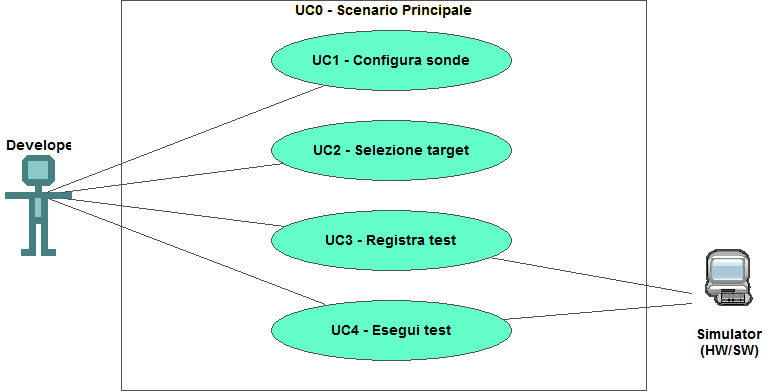
\includegraphics[width=0.9\columnwidth]{usecase/scenario-principale} 
    \caption{Use Case - UC0: Scenario principale}
\end{figure}

\begin{usecase}{0}{Scenario principale}
\usecaseactors{Sviluppatore applicativi}
\usecasepre{Lo sviluppatore è entrato nel plug-in di simulazione all'interno dell'IDE}
\usecasedesc{La finestra di simulazione mette a disposizione i comandi per configurare, registrare o eseguire un test}
\usecasepost{Il sistema è pronto per permettere una nuova interazione}
\label{uc:scenario-principale}
\end{usecase}

\section{Tracciamento dei requisiti}

Da un'attenta analisi dei requisiti e degli use case effettuata sul progetto è stata stilata la tabella che traccia i requisiti in rapporto agli use case.\\
Sono stati individuati diversi tipi di requisiti e si è quindi fatto utilizzo di un codice identificativo per distinguerli.\\
Il codice dei requisiti è così strutturato R(F/Q/V)(N/D/O) dove:
\begin{enumerate}
	\item[R =] requisito
    \item[F =] funzionale
    \item[Q =] qualitativo
    \item[V =] di vincolo
    \item[N =] obbligatorio (necessario)
    \item[D =] desiderabile
    \item[Z =] opzionale
\end{enumerate}
Nelle tabelle \ref{tab:requisiti-funzionali}, \ref{tab:requisiti-qualitativi} e \ref{tab:requisiti-vincolo} sono riassunti i requisiti e il loro tracciamento con gli use case delineati in fase di analisi.

\newpage

\begin{table}%
\caption{Tabella del tracciamento dei requisti funzionali}
\label{tab:requisiti-funzionali}
\begin{tabularx}{\textwidth}{lXl}
\hline\hline
\textbf{Requisito} & \textbf{Descrizione} & \textbf{Use Case}\\
\hline
RFN-1     & L'interfaccia permette di configurare il tipo di sonde del test & UC1 \\
\hline
\end{tabularx}
\end{table}%

\begin{table}%
\caption{Tabella del tracciamento dei requisiti qualitativi}
\label{tab:requisiti-qualitativi}
\begin{tabularx}{\textwidth}{lXl}
\hline\hline
\textbf{Requisito} & \textbf{Descrizione} & \textbf{Use Case}\\
\hline
RQD-1    & Le prestazioni del simulatore hardware deve garantire la giusta esecuzione dei test e non la generazione di falsi negativi & - \\
\hline
\end{tabularx}
\end{table}%

\begin{table}%
\caption{Tabella del tracciamento dei requisiti di vincolo}
\label{tab:requisiti-vincolo}
\begin{tabularx}{\textwidth}{lXl}
\hline\hline
\textbf{Requisito} & \textbf{Descrizione} & \textbf{Use Case}\\
\hline
RVO-1    & La libreria per l'esecuzione dei test automatici deve essere riutilizzabile & - \\
\hline
\end{tabularx}
\end{table}%

    \chapter{Progettazione e codifica}
\label{cap:progettazione-codifica}

\intro{Breve introduzione al capitolo}\\

\section{Tecnologie e strumenti}
\label{sec:tecnologie-strumenti}

Di seguito viene data una panoramica delle tecnologie e strumenti utilizzati.

\subsection*{Tecnologia 1}
Descrizione Tecnologia 1.

\subsection*{Tecnologia 2}
Descrizione Tecnologia 2

\section{Ciclo di vita del software}
\label{sec:ciclo-vita-software}

\section{Progettazione}
\label{sec:progettazione}

\subsubsection{Namespace 1} %**************************
Descrizione namespace 1.

\begin{namespacedesc}
    \classdesc{Classe 1}{Descrizione classe 1}
    \classdesc{Classe 2}{Descrizione classe 2}
\end{namespacedesc}


\section{Design Pattern utilizzati}

\section{Codifica}

    \chapter{Verifica e validazione}
\label{cap:verifica-validazione}

    \chapter{Conclusioni e Sviluppi Futuri}
\label{cap:conclusioni}

\section{Consuntivo finale}
In questo studio, si sono analizzate diverse possibili strategie per alterare il traffico dati in connessioni \emph{QUIC},
con particolare attenzione sulle ritrasmissioni e sulle tecniche per aumentare artificialmente il consumo di dati.
\\\\
I risultati degli esperimenti condotti hanno confermato le ipotesi iniziali, rivelando una serie di metodi efficaci per aumentare il traffico dati. 
Si è evidenziato come un \emph{server} malevolo possa effettivamente incrementare il traffico dati, causando un aumento misurabile del consumo totale del \emph{client}.
In particolare, nel primo esperimento ignorando gli ACK, mentre nel secondo iniettando pacchetti aggiuntivi alla connessione normale. 
I risultati ottenuti suggeriscono che combinando le diverse strategie sperimentate si
potrebbe potenzialmente amplificare ulteriormente l'impatto sull'incremento del traffico. 
Ancora più significativi sono i risultati del terzo esperimento, dove si è evidenziato che anche senza il controllo diretto di \emph{client} o \emph{server}, 
un attaccante può manipolare il traffico dati, causando un aumento del 50\% nel volume di pacchetti trasmessi.
\\\\
Questo studio dimostra come un utente malevolo possa indurre un aumento del traffico dati per l'utente vittima, incrementando di conseguenza il suo consumo di dati e i relativi costi.
Le implicazioni dei risultati ottenuti evidenziano potenziali strategie che potrebbero essere sfruttate per causare danni economici agli utenti o sovraccaricare le reti di comunicazione.
\section{Sviluppi Futuri}
~\\
\indent Nonostante il presente studio si sia concentrato principalmente sull'analisi delle vulnerabilità di \emph{QUIC} e sul loro potenziale sfruttamento per manipolare i sistemi di contabilizzazione del traffico mobile, questa ricerca si inserisce in un contesto più ampio che include anche un'analisi di \emph{MPTCP}.
Un possibile sviluppo futuro potrebbe consistere in un'analisi più dettagliata di quest'ultimo protocollo.
Sarebbe interessante replicare l'approccio utilizzato nell'esperimento uno di \emph{QUIC}, costruendo un server malevolo per \emph{MPTCP},
per confrontare il comportamento dei due protocolli.
\\\\
Un altro possibile sviluppo sarebbe l'estensione della sperimentazione in scenari reali, uscendo dagli ambienti controllati utilizzati finora. 
Condurre esperimenti in contesti reali permetterebbe di valutare l'effettivo impatto delle vulnerabilità individuate. 
Inoltre, questo approccio consentirebbe di analizzare le politiche di contabilizzazione delle ritrasmissioni adottate dai diversi operatori 
e di confrontarli per identificare eventuali differenze nel conteggio del consumo dati.
\\\\
Un approfondimento specifico su \emph{Multipath QUIC (MPQUIC)} sarebbe di grande interesse. 
Introdotto per la prima volta nel 2017 nel paper \emph{"Multipath QUIC: Design and Evaluation"} \cite{article:mpquic},
\emph{MPQUIC} è un'estensione del protocollo \emph{QUIC} che permette agli host di scambiare dati su reti multiple attraverso una singola connessione.
Data la sua natura di estensione di \emph{QUIC},
\emph{MPQUIC} potrebbe presentare vulnerabilità uniche o comportamenti di rete differenti, che meriterebbero un approfondimento.


    \appendix
    \chapter{Appendice}

\begin{table}[h!]
    \caption*{Elenco completo delle varianti Esperimento 1}
    \resizebox{\textwidth}{!}{ % Adatta la tabella alla larghezza del testo disponibile
        \begin{tabular}{|c|c|c|c|c|c|}
            \hline
            \textbf{Nome} & \textbf{Connection Close} & \textbf{ACK Ignored} & \textbf{timeThreshold} & \textbf{packetThreshold} & \textbf{amplificationFactor} \\
            \hline
            Retransmission - 1  & Ignored & All & 9.0/8  & 3 & 3 \\
            \hline
            Retransmission - 1.1  & Ignored & All & 9.0/8  & 1 & 1 \\
            \hline
            Retransmission - 2 & Not Ignored & All & 9.0/8  & 3 & 3 \\
            \hline
            Retransmission - 4 & Not Ignored & 1/2  & 9.0/8  & 3 & 3\\
            \hline
            Retransmission - 4.1 & Not Ignored & 1/2 & 9.0/8  & 5 & 5 \\
            \hline
            Retransmission - 4.2 & Not Ignored & 1/2 & 9.0/8  & 10 & 3 \\
            \hline
            Retransmission - 5 & Ignored & 1/2 & 9.0/8  & 3 & 3 \\
            \hline
            Retransmission - 5.1 & Ignored & 1/2 & 9.0/8  & 5 & 5 \\
            \hline
            Retransmission - 5.2 & Ignored & 1/2 & 9.0/8  & 10 & 3 \\
            \hline
            Retransmission - 5.2 & Ignored & 1/2 & 9.0/8  & 20 & 3 \\
            \hline
            Retransmission - 6 & Not Ignored & 1/2 & 9.0/8  & 1 & 1 \\
            \hline
            Retransmission - 7 & Not Ignored & 2/3 & 9.0/8  & 3 & 3 \\
            \hline
            Retransmission - 8 & Not Ignored & 4/5 & 9.0/8  & 3 & 3 \\
            \hline

        \end{tabular}
    }
\end{table}

\begin{table}[h!]
    \centering
    \caption*{Elenco completo delle varianti Esperimento 2}
    \begin{tabular}{|c|c|c|}
        \hline
        \textbf{Nome} & \textbf{Worker} & \textbf{Packet/s} \\
        \hline
        inject - 1 & 6 & 1000 \\
        \hline
        inject - 2 & 6 & 2000 \\
        \hline
        inject - 3 & 8 & 1000 \\
        \hline
        inject - 4 & 8 & 2000 \\
        \hline
        inject - 5 & 6 & 3000 \\
        \hline
        inject - 6 & 6 & 4000 \\
        \hline
        inject - 7 & 8 & 3000 \\
        \hline
        inject - 8 & 8 & 4000 \\
        \hline
        inject - 9 & 4 & 3000 \\
        \hline
        inject - 10 & 4 & 4000 \\
        \hline
        inject - 11 & 4 & 5000 \\
        \hline
    \end{tabular}
\end{table}

\begin{table}[h!]
    \centering
    \caption*{Elenco completo delle varianti Esperimento 3}
    \begin{tabular}{|c|c|}
        \hline
        \textbf{Nome} & \textbf{ACK Packet} \\
        \hline
        spurious - 1  & All \\
        \hline
        spurious - 2 & 1/2 \\
        \hline
        spurious - 3 & 2/3 \\
        \hline
        spurious - 4 & 4/5 \\
        \hline
        spurious - 5 & 7/8 \\
        \hline
        spurious - 6 & 9/10 \\
        \hline
        spurious - 7 & 19/20 \\
        \hline
    \end{tabular}
\end{table}

\begin{table}[h!]
    \centering
    \caption*{Risultati Esperimento 1}
    \begin{tabular}{|c|c|c|}
        \hline
        \textbf{Nome} & \textbf{Consumo (Mb)} & \textbf{Numero Pacchetti} \\
        \hline
        retransmission - 1 & ~13 & 18030 \\
        \hline
        retransmission - 2 & ~15 & 18000 \\
        \hline
        retransmission - 4 & ~58 & 65500 \\
        \hline
        retransmission - 5 & ~29 & 35900 \\
        \hline
    \end{tabular}
\end{table}

\begin{table}[h!]
    \centering
    \caption*{Risultati Esperimento 2}
    \begin{tabular}{|c|c|c|c|}
        \hline
        \textbf{Nome} & \textbf{Durata} & \textbf{Consumo (Mb)} & \textbf{Numero Pacchetti} \\
        \hline
        inject - 1 & ~30s & ~272 & 198482 \\
        \hline
        inject - 2 & ~30s & ~566 & 396429 \\
        \hline
        inject - 3 & ~30s & ~407 & 535913 \\
        \hline
        inject - 4 & ~30s & ~753 & 543020 \\
        \hline
    \end{tabular}
\end{table}

\begin{table}[h!]
    \centering
    \caption*{Risultati Esperimento 3}
    \begin{tabular}{|c|c|c|}
        \hline
        \textbf{Nome} & \textbf{Consumo (Mb)} & \textbf{Numero Pacchetti} \\
        \hline
        spurious - 1 & - & - \\
        \hline
        spurious - 2 & ~5.9 & 4700 \\
        \hline
        spurious - 3 & ~6.6 & 5377 \\
        \hline
        spurious - 4 & ~7.7 & 6226 \\
        \hline
    \end{tabular}
\end{table}



    \backmatter
    \printglossary[type=\acronymtype, title=Acronimi e abbreviazioni, toctitle=Acronimi e abbreviazioni]
    \printglossary[type=main, title=Glossario, toctitle=Glossario]

    \cleardoublepage
\chapter{Bibliografia}

\nocite{*}

% Print book bibliography
\printbibliography[heading=subbibliography,title={Riferimenti bibliografici},type=book]

% Print site bibliography
\printbibliography[heading=subbibliography,title={Siti web consultati},type=online]

\end{document}
